\chapter{Implementation}

Interfacing: Clean interfaces are generated throughout the model. Enabling a standardized state vector x. Meaning that A remains standardized for any aircraft while B, U and L need to be adjusted for any changes to the aircraft or sensor data.

The integration step may be omitted in early design stages since the necessary equations and equilibriums of Forces and Moments could only be modelled linearly while neglecting various unknown factors like shifting CG due to fuel burn, actual Inertia of Aircraft and aicraft mass. Hence, this step may be implemented if time allows it.

\section{Examining Height and altitude}

As seen in~\ref{fig:gps_diff} gps altitudes have a base mean value of difference of about 3-4 meters. During flight level changes the base level changes significantly. Further investigation is needed how these changes may arise.

One possible approach would be considering different placements of gps antennas within the airframe. since the IMAR's position is precisely known and lies around the center of gravity but the ASCB's gps position is not known exactly the process is not facilitated. However using the process of lever arms the position could be roughly estimated and compensated from the altitude difference in figure \ref{fig:gps_diff}.

\begin{figure}[h]
         \centering
         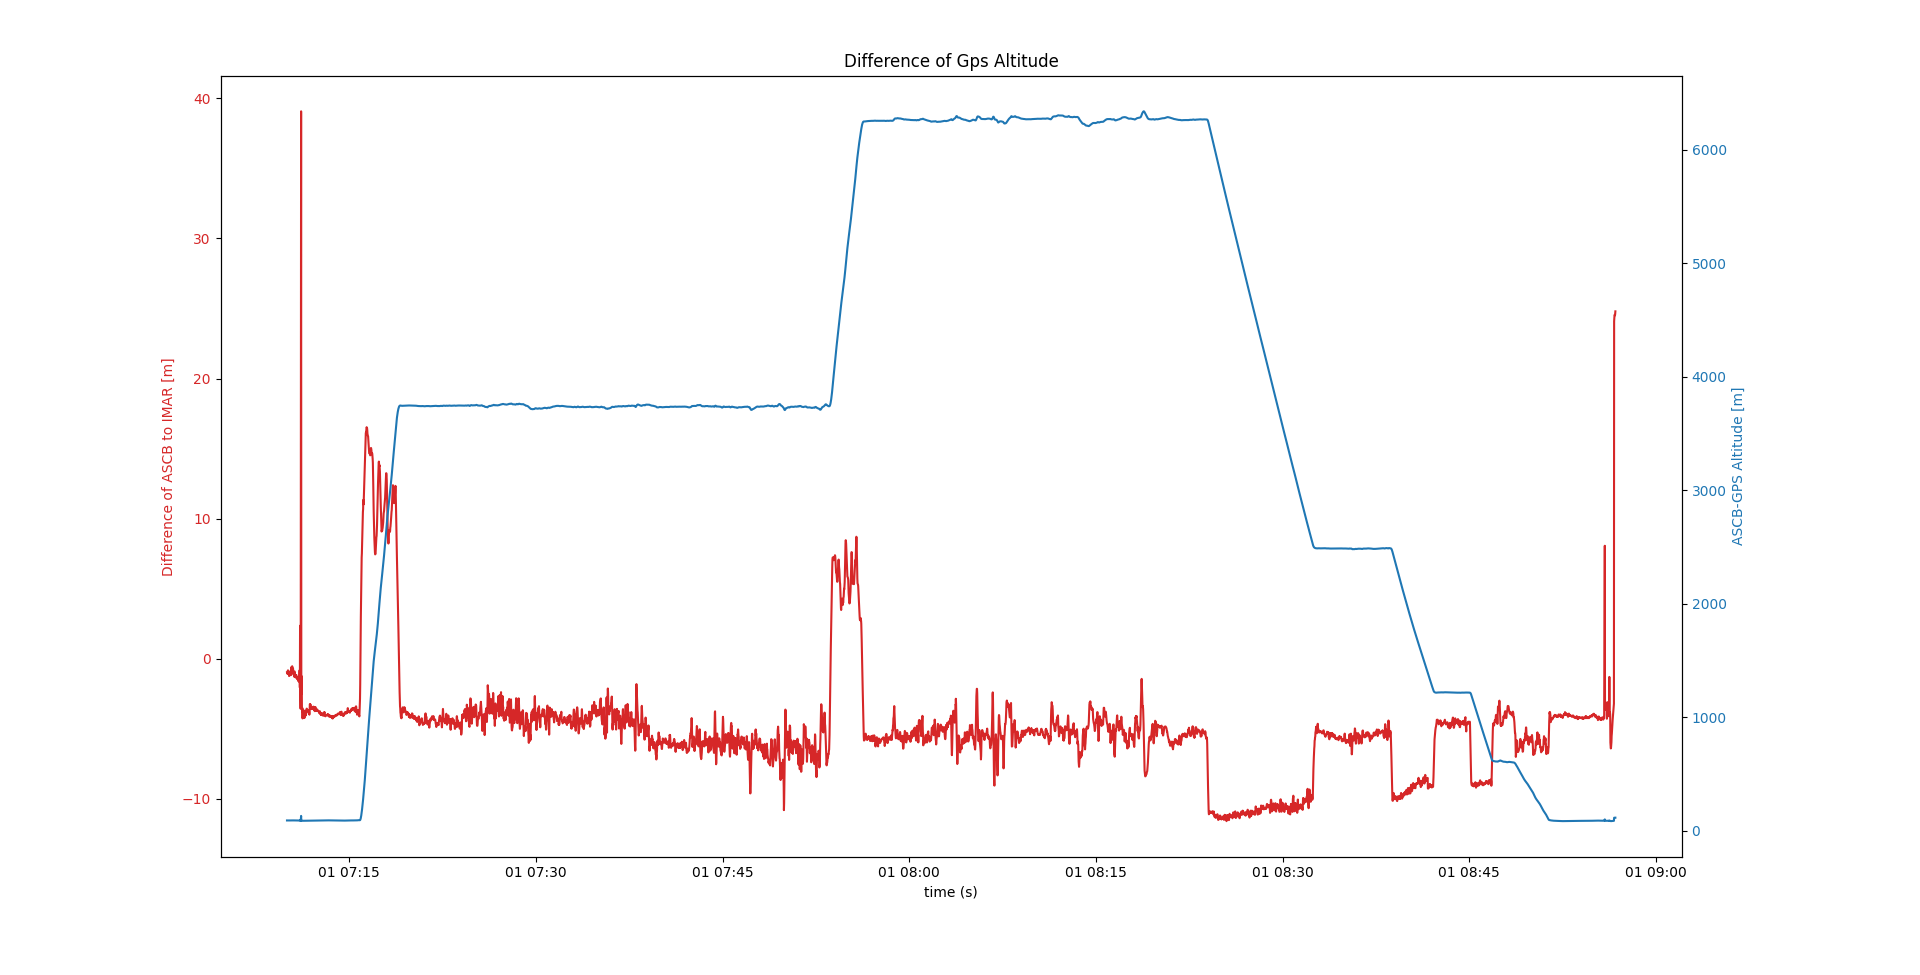
\includegraphics[width=.8\textwidth]{gps_difference_imar_ascb}
         \caption{GPS difference for the aircraft base platform (ASCB) as well as experimental sensor (IMAR)}
         \label{fig:gps_diff}
\end{figure}

Another incurring deviation is investigating the ~40m/150ft offset for gps altitudes. Possible causes may be Uncorrected Ellipsoid gnss altitudes. However, this appears unlikely since generally the offset in the region would be added and not subtracted [further investigation needed].

